\documentclass[12pt,a4paper]{article}
\usepackage{times}
\usepackage{mathptmx}
\usepackage{setspace}
\usepackage[utf8]{inputenc}
\usepackage[french]{babel}
\usepackage[T1]{fontenc}
\usepackage{amsmath}
\usepackage{amsfonts}
\usepackage{amssymb}
\usepackage{makeidx}
\usepackage{graphicx}
\usepackage{lmodern}
\usepackage{index}
\usepackage{diagbox}
\usepackage{multirow}

%\usepackage{hyperref}
\newcommand{\HRule}{\rule{\linewidth}{0.5mm}}
%\usepackage{kpfonts}
\usepackage{fourier}
\usepackage[left=2cm,right=2.5cm,top=2.5cm,bottom=2.5cm]{geometry}
\author{Sarah Kaddah}
\title{Rapport de stage}

%%%%%%%%%%Interligne
\renewcommand{\baselinestretch}{1.5}
\begin{document}
%%%%%%%%%%%%%%%%%%%%%%%%%%%%%%%%%%%%%%%%%%%%%%%%%%%%%%%%%%%%%%%%%
%%%%%%%%%%%%%%%%%%%%%%1ere page%%%%%%%%%%%%%%%%%%%%%%%%%%%%%%%%%%
%%%%%%%%%%%%%%%%%%%%%%%%%%%%%%%%%%%%%%%%%%%%%%%%%%%%%%%%%%%%%%%%%
%%%%%%%%%%%%%%%%%%%%%%%%%%%%%%%%%%%%%%%%%%%%%%%%%%%%%%%%%%%%%%%%%
\begin{titlepage}
  \begin{sffamily}
  \begin{center}
	\large{Université Paris Diderot - Paris 7 \hfill 2017-2018} \bigskip
	\center{\LARGE{Master 2 Biologie-Informatique/ Bioinformatique}}
	
\begin{tabular}{c}
\\ \\ \\
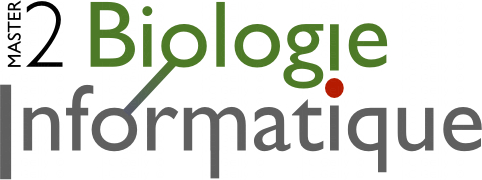
\includegraphics[scale=0.3]{img/m2.png}
\end{tabular}
\hfill
\begin{tabular}{c}
\\

\includegraphics[scale=0.1]{img/p7.png}
\end{tabular}

%%%%%%%%% Title    
    \HRule \\[0.2cm]
    { \huge \bfseries \center{Etude de la fonction et des mécanismes d'évolution des séquences répétées centromériques chez les Primates}\\[0.4cm] }
    \HRule \\%[2cm]
%%%%%%%%Centre de la page    
\begin{center}\LARGE{\textbf{Sarah Kaddah}}\end{center}%~\\[0.1cm]

%%%%%%%%% Bottom of the page
\begin{center}\Large{Tuteur: Lo\"{i}c Ponger}\end{center}~\\%[0.5cm]
\center{\large{Structure et Instabilité des Génomes}}
\center{\large{ MNHN - CNRS UMR 7196 / INSERM U1154 - Sorbonne Universités}}\\%[1cm]
Muséum national d'Histoire naturelle, 43 rue Cuvier 75005 PARIS \\ [1cm]
%	\begin{center}
%		
\includegraphics[scale=0.2]{img/mnhn.jpg} \hfill
%		
\includegraphics[scale=0.08]{img/cnrs.png} \hfill
%		
\includegraphics[scale=0.08]{img/inserm.jpg}
%	\end{center} 

\begin{tabular}{cc}
 \hspace*{2.5cm} &  

\includegraphics[scale=0.2]{img/mnhn.jpg}
\end{tabular}
\hfill
\begin{tabular}{c}

\includegraphics[scale=0.08]{img/inserm.jpg}
\end{tabular}
\hfill
\begin{tabular}{cc}

\includegraphics[scale=0.08]{img/cnrs.png} &
\hspace*{2.5cm}
\end{tabular}

%%%%%%%%% END
  \end{center}
  \end{sffamily}
\end{titlepage}
%%%%%%%%%%%%%%%%%%%%%%%%%%%%%%%%%%%%%%%%%%%%%%%%%%%%%%%%%%%%%%%%%%
%%%%%%%%%%%%%%%%%%%%%Remerciements%%%%%%%%%%%%%%%%%%%%%%%%%%%%%%%%
%%%%%%%%%%%%%%%%%%%%%%%%%%%%%%%%%%%%%%%%%%%%%%%%%%%%%%%%%%%%%%%%%%

\section*{\begin{center}Remerciements\end{center}}~\\[0.2cm]
\addcontentsline{toc}{section}{Remerciements}
Merci à Namrod pour toute la partie sur la bibliographie. Retrouvez ses questions FAQ qui ont permis la rédaction de cette partie.\\
\noindent Merci à f-leb, LittleWhite et Metalman pour leurs conseils et la relecture.
\noindent Merci à ced et jacques\_jean pour la correction orthographique et typographique.
\thispagestyle{empty}

%%%%%%%%%%%%%%%%%%%%%%%%%%%%%%%%%%%%%%%%%%%%%%%%%%%%%%%%%%%%%%%%%%
%%%%%%%%%%%%%%%%%%%Table des matières%%%%%%%%%%%%%%%%%%%%%%%%%%%%
%%%%%%%%%%%%%%%%%%%%%%%%%%%%%%%%%%%%%%%%%%%%%%%%%%%%%%%%%%%%%%%%%

\newpage
\tableofcontents
\setcounter{page}{0}
\thispagestyle{empty}
\newpage 
%%%%%%%%%%%%%%%%%%%%%%%%%%%%%%%%%%%%%%%%%%%%%%%%%%%%%%%%%%%%%%%%
%%%%%%%%%%%%%%%%%%%%Introduction%%%%%%%%%%%%%%%%%%%%%%%%%%%%%%%%
%%%%%%%%%%%%%%%%%%%%%%%%%%%%%%%%%%%%%%%%%%%%%%%%%%%%%%%%%%%%%%%% 

\section{Introduction}
\subsection{Le centromère}
Le centromère est une structure chromatinienne caractérisé par la présence de CENP-A. Cette protéine, très conservée au cours de l'évolution, est un variant de l'histone H3. Son rôle est de fixer la position du kinétochore par un mécanisme encore peu connu. En effet, le centromère est le site d'assemblage du kinétochore, un ensemble d'ADN et de protéines. Il permet l'attachement du fuseau mitotique pour la ségrégation des chromosomes durant la division cellulaire chez les eucaryotes. Le centromère et les protéines impliquées sont relativement bien conservés. Au contraire, l'ADN sous-jacent est très diversifié et l'organisation varie d'un taxon à l'autre. Cependant, une caractéristique commune est retrouvée chez toute les espèces: de l'ADN centromérique répété en tandem nommé ADN satellite. Ces répétitions sont issues d'événements d'amplification, tels les crossovers inégaux, la conversion de gènes, les cercles roulants ou la transposition de séquences.[Malik and Henikoff, 2002; Plohl et al. 2012]
Ces séquences représentent 5\% du génome. Les répétitions s'étendent de 7pb à 3,2kb avec des séquences de 145-180kb le plus souvent.  

\subsection{L'ADN $\alpha$-satellites}
L'ADN satellite chez les Primates est connu sous le nom d'$\alpha$-satellite. Ces séquences centromériques répétées en tandem sont riches en AT. 

Des études chez l'Homme propose un modèle évolutif. La répartition des $\alpha$-satellites suivrait une répartition spécifique selon l'âge des familles. Les familles les plus jeunes s'insèrent au cœur du centromère, repoussant les familles les plus anciennes jusqu'aux regions voisines, appelé péri-centromère.\\

Un monomère a une longueur de 171pb et il peut être répété des milliers de fois. Les monomères peuvent être répartis en famille selon leur similarité, les séquences ayant un taux d'identité supérieur à 70\%. Ces séquences ont soit une organisation monomérique soit une organisation en répétition d'ordre supérieur (Fig. 1). Dans le premier cas, les séquences d'une même famille sont répétés en tandem. Dans le deuxème cas, une suite de monomères appartenant à différentes familles forme une unité, qui elle est répétée en tandem. 

Ces séquences peuvent avoir un site de liaison à la protéine centromérique CENP-B un motif spécifique de 17pb. Cette protéine, qui reconnaît et se fixe sur l'ADN, serait présente chez de nombreuses familles de Primates. La protéine pJ$\alpha$, une protéine peu caractérisée, reconnaît un motif qui remplace celui de CENP-B.

Les $\alpha$-satellites ont essentiellement été étudiées chez l'homme. Modèle évolutif avec les centromères en expansion. Une hypothèse concernant l'âge des séquences découle de ces recherches: les séquences les plus récentes apparaissent au coeur du centromères, déplançant les plus anciennes au péricentromère. D'autres études chez le gorille ont été faites. Le rôle des $\alpha$-satellites est encore mal connu. 

\begin{figure}
	\center
		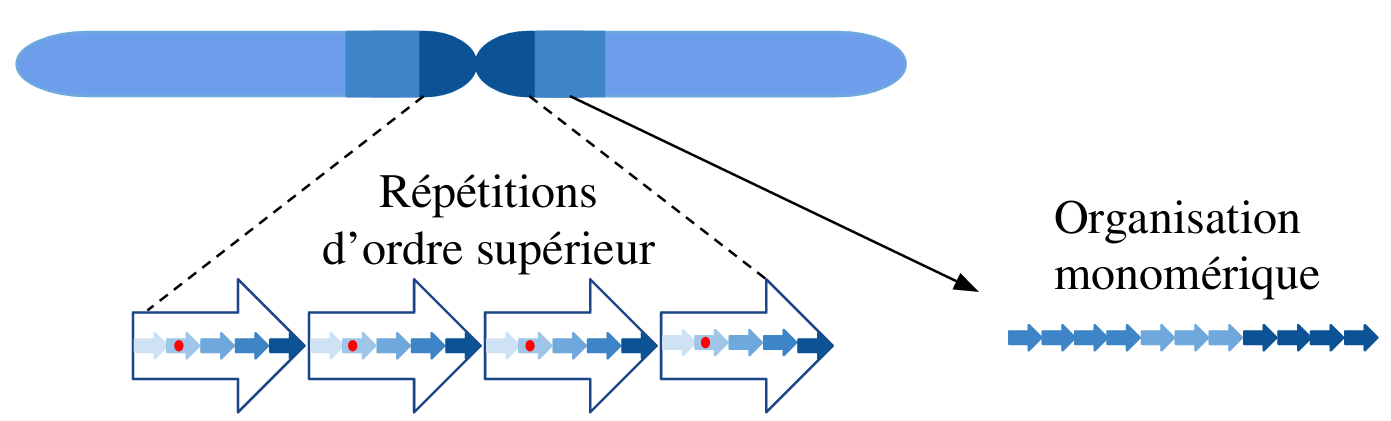
\includegraphics[height=3.5cm, width=12cm]{img/AS_organization.png}
		\caption{\textbf{Organisation spatiale des $\alpha$-satellites:} Le coeur du centromère (bleu foncé) est organisé en répétition d'ordre supérieur. Le péricentromère(bleu clair) a une organisation monomérique. Un monomère d'une même famille est représenté par une petite flèche de même couleur. Les points rouges représentent les sites de fixation à CENP-B ou pJ$\alpha$.}
\end{figure}

\subsection{Le sujet de stage}

Peu d'informations sur les $\alpha$-satellites figurent chez les autres espèces de primates, et aucune relation inter-espèce n'a été réalisée. Les études se basant sur un séquençage haut-débit est appliqué chez l'homme (cité ci-dessus) et chez le Gorille. [compléter] L'équipe d'accueil de mon stage "ADN répété, Chromatine, Evolution" ou ARChE, a récemment développé une approche de séquençage haut débit, ciblée sur les séquences $\alpha$-satellites chez deux espèces: \textit{Cercopithecus solatus} et \textit{Cercopithecus pogonias}.

Les méthodes basées sur l'alignement et la phylogénie sont très limitées pour étudier ces séquences. Elles ne permettent pas de traiter des jeux de données conséquents, or un monomère peut avoir des milliers de copies dans un seul génome. De plus, ces méthodes non-objectives ne permettent pas de faire des comparaisons entre espèces.

Pour remédier à ce problème, une méthode de classification automatisée des $\alpha$-satellites a été implémentée en R en 2016, puis améliorée en 2017 en Python dans le laboratoire. Ce programme permet de traiter des centaines de milliers de séquences, quelque soit le nombre ou la taille des familles. De plus, cette méthode est objective et peut être appliquée à plusieurs espèces, permettant ainsi une comparaison inter-espèce des familles $\alpha$-satellites. 

L'objectif de ce stage est de comprendre la fonction des $\alpha$-satellites, notamment en caractérisant les familles issues de cette classification chez quatre espèces proches de primates. Parmi ces espèces, les deux Cercopithèques séquencés dans le laboratoire permettront d'avoir un avis objectif sur la méthode de classification.  Dans une deuxième temps, les mécanismes d'évolution pourront être déduits à partir d'une comparaison inter-espèce révélant les différences et les familles communes. 

%%%%%%%%%%%%%%%%%%%%%%%%%%%%%%%%%%%%%%%%%%%%%%%%%%%%%%%%%%%%%%%%%
%%%%%%%%%%%%%%%%%%%%%%M & M%%%%%%%%%%%%%%%%%%%%%%%%%%%%%%%%%%%%%%
%%%%%%%%%%%%%%%%%%%%%%%%%%%%%%%%%%%%%%%%%%%%%%%%%%%%%%%%%%%%%%%%% 
\section{Matériel et méthode}
\subsection{Choix des espèces}

	\begin{figure}
		\center
		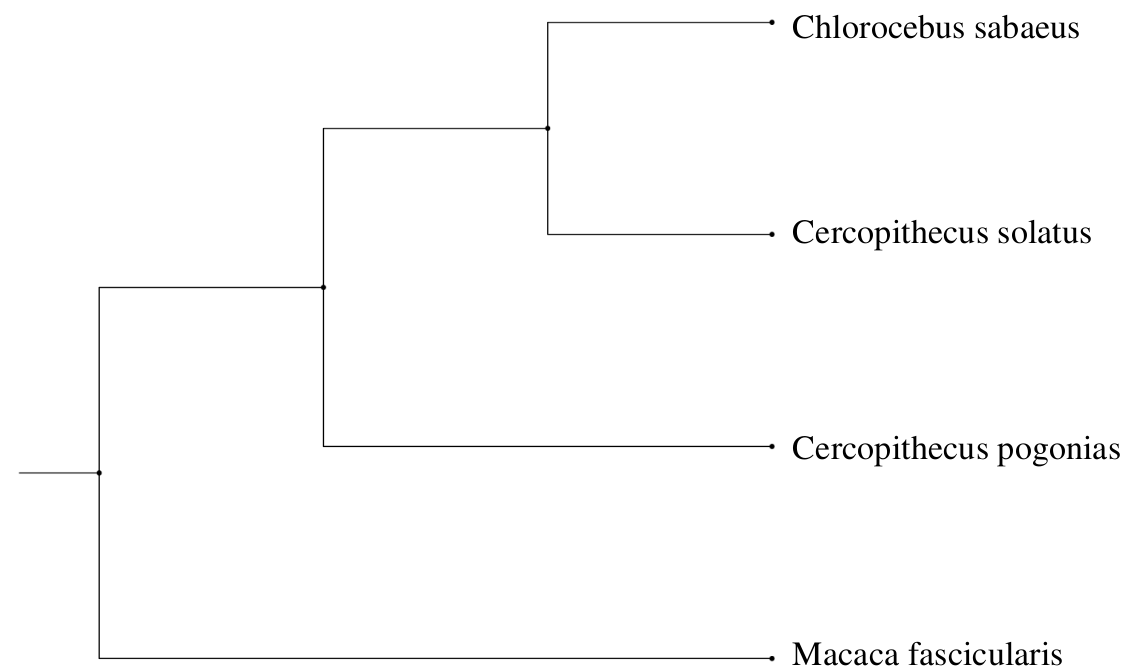
\includegraphics[height=4.5cm, width=7cm]{img/arbre_especes.png}
		\caption{\textbf{Arbre phylogénétique des espèces analysées.}\cite{Cacheux_evolution}
		\label{fig:arbre_presentation}}
	\end{figure}

Les critères de sélection dépendent de la disponibilité des séquences de qualité. Deux espèces du laboratoire sont choisies, le \textit{C. solatus} et \textit{C. pogonias}, et deux espèces proches (Fig. \ref{fig:arbre_presentation}), le \textit{Macaca fascicularis} et le \textit{Chlorocebus sabaeus}.  

\subsection{Méthode de classification}
	\subsubsection{Principe}
Cette méthode \cite{rapport_florence} répartit des séquences $\alpha$-satellites en familles selon la similarité. La classification est hiérarchique dichotomique. Au départ, une table contenant les fréquences des 5-mers est calculée pour chaque monomère. Ensuite une boucle itérative est exécutée pour séparer les séquences en groupes tant que les nouveaux groupes formés sont divisibles.

	\subsubsection{Répartition itérative}
Une Analyse en Composante Principale (ACP) est effectuée sur la table des fréquences des 5-mers afin de réduire les dimensions du jeu de données et d’obtenir des variables indépendantes. Des distances euclidiennes sont calculées entre toutes les paires de séquence dans l’espace défini par les premières composantes de l’ACP. 

A partir du calcul de distance, les séquences sont séparées en deux classes en utilisant la classification hiérarchique basée sur la méthode de Ward. Cette méthode maximise l’inertie interclasse. La classification hiérarchique fait un usage important de la mémoire. Par conséquent, pour traiter des jeux de données importants de plus de 100 000 séquences, l’Analyse Discriminante Linéaire , une méthode d’apprentissage, est utilisée sur un sous jeu de données formé par de 100 000 séquences tirées aléatoirement, dans ces analyses. Le modèle construit est alors appliqué sur toutes les séquences.

	\subsubsection{Double-validation d'un sous-groupe}
Le premier critère de validation est la taille du sous-groupe. Si un groupe atteint 100 séquences, il n'est pas redivisé. Le deuxième critère de validation s'appuie sur le \textit{matepair}. Ce terme correspond à la proportion de monomères ayant son plus proche voisin dans la même classe, se basant sur les distances euclidiennes calculées auparavant. Des valeurs \textit{matepairs} élevées (proches de 1) indiquent des sous-groupes bien homogènes et séparés validant la classification tandis qu’un seuil \textit{matepair} plus faible (proche de 0) entraîne plus de classes.

Un seuil de \textit{matepair} est fixé à 0.90, pour avoir des groupes homogènes. Si au moins une des valeurs de \textit{matepair} est au-dessous de ce seuil, les sous-groupes sont considérés comme formant un seul groupe et le groupe initial est sauvegardé comme une famille unique. Si les \textit{matepairs} sont au-dessus d’un certain seuil, les deux sous-groupes sont ajoutés séparément à la file pour être potentiellement redivisés ultérieurement.

	\subsection{Analyse des séquences}
L'alignement des séquence est fait avec muscle \cite{Edgar2004} et SeaView \cite{Gouy2009}, un éditeur d'alignements multiples. 
La phylogénie est construite avec la méthode du maximum de vraisemblance (PhyML) \cite{Guindon2009a}. Le modèle F84 est utilisé pour la construction de l'arbre. Le support de branche est aLRT (SH-like). La fréquence d'équilibre nucléotidique est optimisée. Le ratio de transition et de transversion est fixé à 4. Aucun site est considéré comme invariable. Le taux de variation à travers le site est optimisé. Les opérations de recherche d'arbre est NNI et l'arbre de départ est défini avec la méthode de Neighbor-Joining \cite{Saitou1987} avec une topologie optimisée.
Les consensus sont obtenus avec des scripts développés par l'équipe. Les motifs CENP-B (TTCGTTGGAA[AG]CGGGA), PJ$\alpha$ (TTCCTTTT[CT]CACC[AG]TAG) et pK$\beta$ (CTATAGGGCCAAAGGAA) ont été identifiés avec le logiciel fuzznuc (package EMBOSS) \cite{Rice2000} et en autorisant 2 différences au maximum par rapport au consensus.

%###########################################################################################################
\section{Résultat}
	\subsection{Caractérisation intraspécifique des familles}
			\subsubsection{Identification des familles}
		
		\begin{table}
			\center
			\begin{tabular}{|c|c|c|c|c|}
   			\hline
  			\textbf{Espèce} & \textit{C. solatus} & \textit{C. pogonias} & \textit{C. sabaeus} & \textit{M. fascicularis}\\
		    \hline
   			\textbf{Nb. seq. au total} & 105 529 & 112 902 & 29 842 & 235 535 \\
   			\hline
   			\textbf{Nb. fam.} & 564 & 132 & 338 & 3694\\
   			\hline
   			\textbf{Nb. grandes fam.} & 12 & 13 & 43 & 114\\
   			\hline
   			\textbf{\% seq. ignorées} & 3.97 & 1.29 & 10.89 & 11.06\\
   			\hline
			\end{tabular}
			\caption{Résumé du jeu de données et des résultats préliminaires de la classification.}
			\label{tab_res}
		\end{table}
		
		\begin{figure}
			\center
			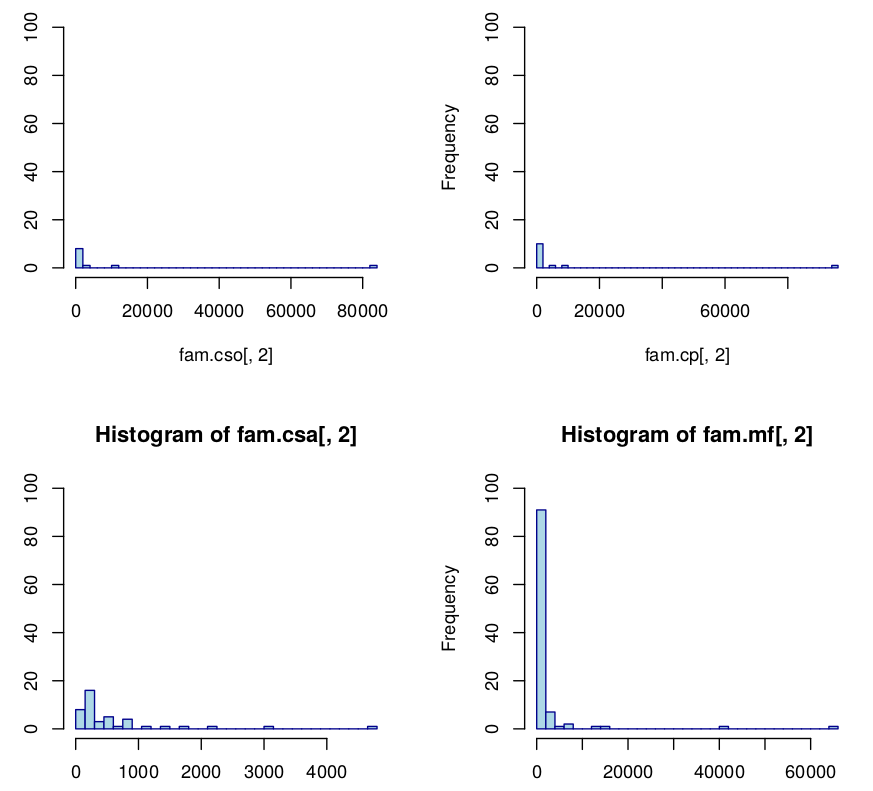
\includegraphics[scale=0.45]{img/distribution_familles.png}
			\caption{\textbf{Distribution des familles en fonction de la taille.}}
			\label{dist_fam} 
		\end{figure}

	A l'issue de la classification, seules les familles ayant plus de 100 séquences, qualifiées de grandes familles, sont conservées pour l'analyse. Le nombre de familles conservées diminue considérablement après élimination des petites familles (<100 séquences) mais ces familles ne représentent que 11\% du jeu de données au plus (Tableau \ref{tab_res}). Les \textit{C. solatus} et \textit{C. pogonias} ont une dizaine de familles, \textit{C. sabaeus} en a 43, et le \textit{M. fascicularis} en a 114. Malgré le nombre de familles qui diffère d'une espèce à l'autre, la distribution des familles est similaire chez les quatre espèces. Les plus petites familles sont très nombreuses et et la fréquence diminue quand la taille augmente (Figure \ref{dist_fam}). Le \textit{C. solatus} possède une grande famille de 80 000 séquences, \textit{C. pogonias} de 94 000 séquences, \textit{M. fascicularis} possède quatre familles de plus de 10 000 séquences. La plus grande famille du \textit{C. sabaeus} fait 5000 séquences. Ces familles se démarquent des autres familles par leur taille.

		\begin{figure}	
			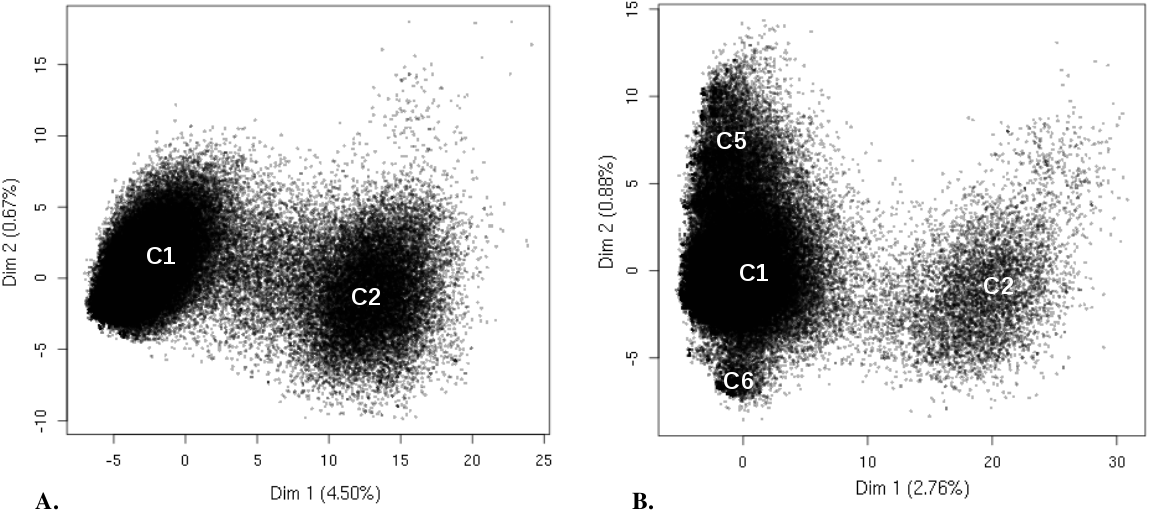
\includegraphics[scale=0.4]{img/ACP_experimental.png}  \\
			\caption{\textbf{Caractérisation visuelle des familles $\alpha$-satellite chez \textit{C. solatus} et \textit{C. pogonias} à partir d'une ACP:}Le nom des familles est indiqué sur les graphiques. Un point représente un monomère. \textbf{A.} \textit{C. solatus}. \textbf{B.} \textit{C. pogonias}.}
			\label{fig:ACP_exp} 
	\end{figure}	
	
	Les espèces \textit{C. solatus} et \textit{C. pogonias} sont analysées dans un premier temps pour comparer la classification automatisée avec la classification expérimentale, une méthode visuelle établie d'après une ACP (Fig. \ref{fig:ACP_exp}).Expérimentalement, 6 familles $\alpha$-satellites ont été déterminées chez les Cercopithèques. Ces deux espèces partagent deux grandes familles monomériques, C1 et C2, et deux familles formant un dimère, C3-C4, de l'ordre d'une centaine de séquences chacune. Le \textit{C. pogonias} possède les familles supplémentaires C5 et C6.\\
		\begin{table}
			\center
			\begin{tabular}{|c|c|c|}
	    	\hline
			\backslashbox{\bf{Fam. exp.}}{\bf{Espèces}} & \textit{C.solatus} & \textit{C.pogonias}\\
			\hline
			C1 &  1  & 10\\
			\hline
			C2 & 11  & 1 \\
			\hline
			C3 & (1) & 1 \\
			\hline
			C4 & (1) & (1) \\
			\hline
			C5 & - 	 &  1 \\
			\hline
			C6 & -   &  0 \\
			\hline
		\end{tabular}
		\caption{\textbf{Résumé du tableau de contingence:} Comptage des familles issues de la classification et leur répartition théorique dans les familles expérimentales (C1 à C6). Les valeurs entre parenthèse sont des petites familles (< 100 séquences) qui ne sont pas prises en compte dans le reste des analyses.}
		\label{tab_count_fam}
	\end{table}	
	Bien que le nombre de grandes familles soit relativement proche entre ces deux espèces, les résultats diffèrent significativement (Tableau \ref{tab_count_fam}). Toutes les familles chez le \textit{C. solatus} sont retrouvées: 11 familles forment la famille C2, une famille forme la famille C1 et les familles C3 et C4 sont retrouvées dans des petites familles d'environ 80 séquences chacune. Chez \textit{C. pogonias}, toutes les familles sont retrouvées sauf la famille C6. La famille C1 est répartie en 10 familles, les familles C2, C3 et C5 sont retrouvées entièrement, la famille C4 est également retrouvée sous la forme d'une petite famille de 86 séquences. Chez le \textit{C. solatus}, la famille C2 est divisée en plusieurs familles et la famille C1 est retrouvée dans une seule famille. La situation inverse est retrouvée  chez \textit{C. pogonias}.
		\begin{figure}	
			\begin{tabular}{cc|cc}
				  & \textit{C. solatus} &  &  \textit{C. pogonias}\\
		\textbf{A} & 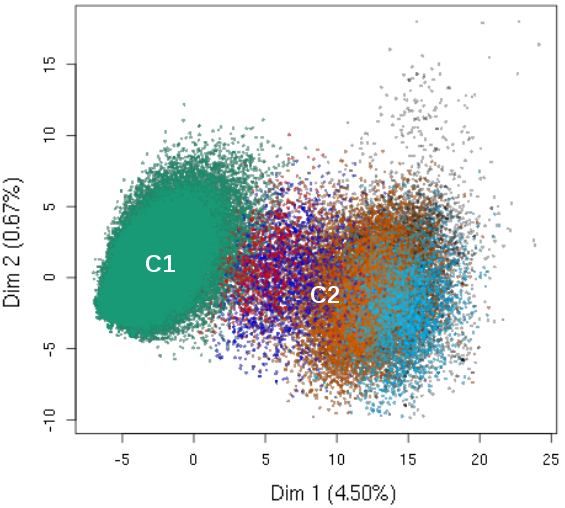
\includegraphics[scale=0.35]{img/solatus_ACP1.png} & \textbf{C} & 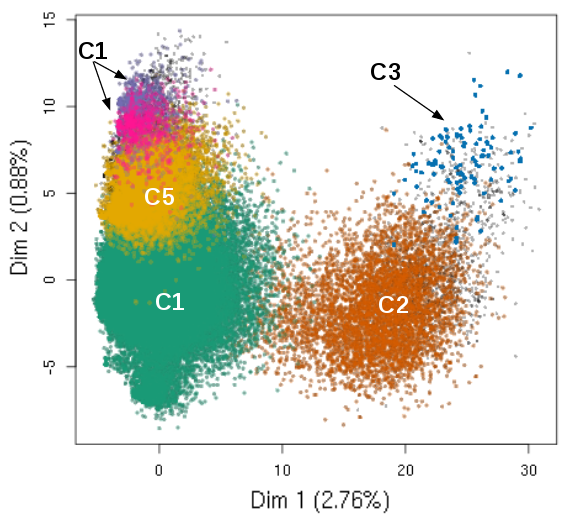
\includegraphics[scale=0.35]{img/pogonias_ACP1.png} \\
		\textbf{B} & 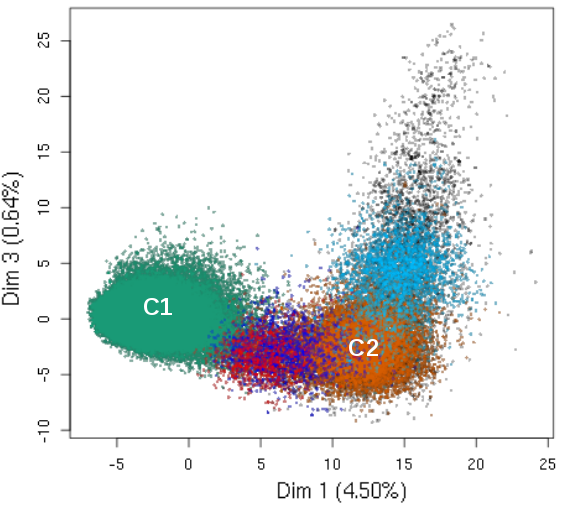
\includegraphics[scale=0.35]{img/solatus_ACP2.png} &  \textbf{D} & 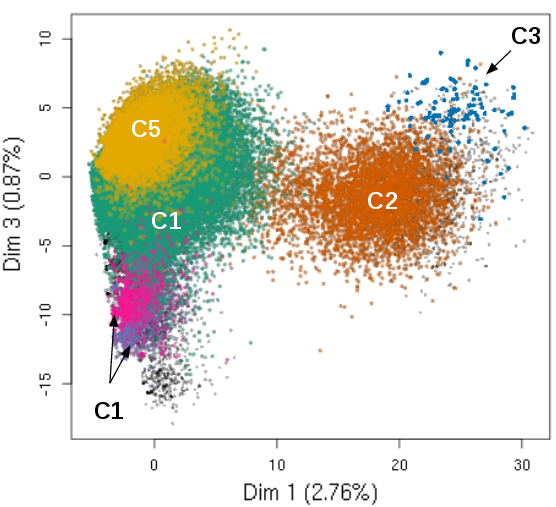
\includegraphics[scale=0.35]{img/pogonias_ACP2.png} \\
		\textbf{E} & 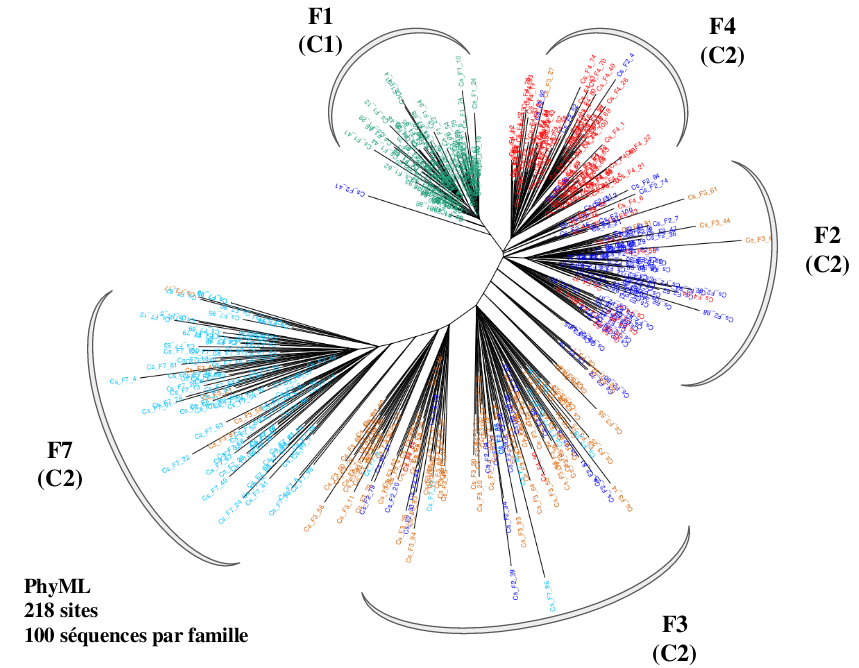
\includegraphics[scale=0.20]{img/tree_solatus.png} & \textbf{F} & 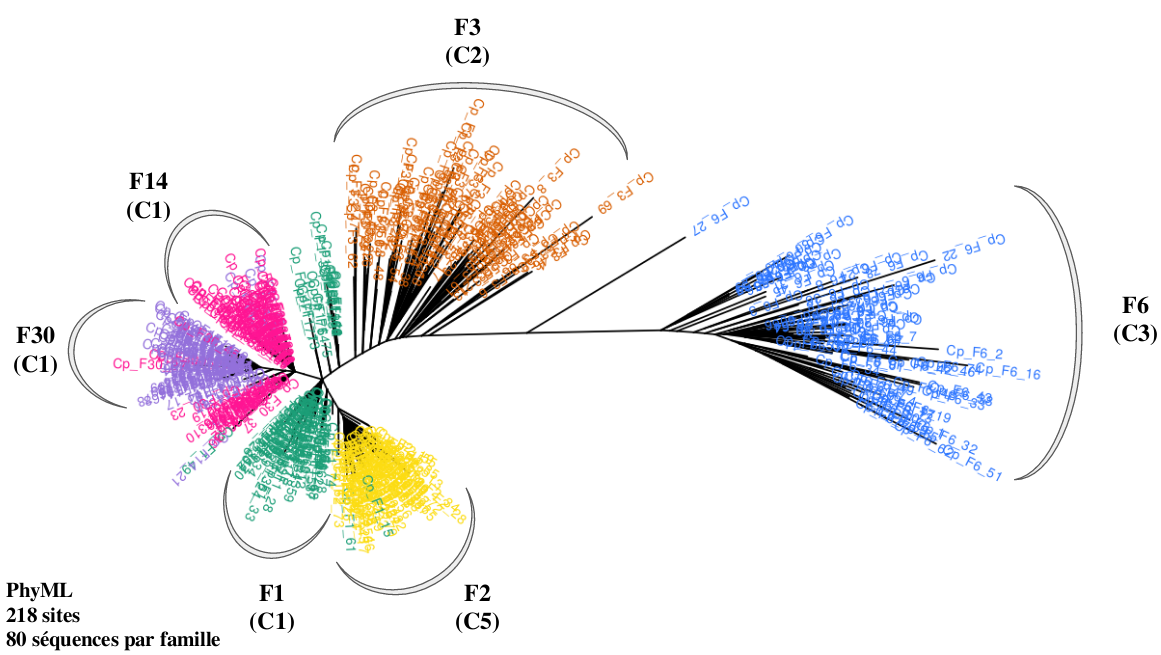
\includegraphics[scale=0.20]{img/tree_pogonias.png} \\
	\end{tabular}
	\caption{\textbf{Représentation des plus grandes familles issues de la classification automatisée:} Ces familles sont superposées sur les représentations de l'ACP des 5-mers.
	\textbf{A.} Composantes 1 et 2 de l'ACP. Les familles qui correspondraient à C1 sont en vert, C2 en orange, rouge, bleu et turquoise.  \textbf{B.} Composantes 1 et 3 de l'ACP. 
	\textbf{C.} Composantes 1 et 2 de l'ACP. Les familles qui correspondraient à C1 sont en vert, violet et rose, C2 en orange, C4 en bleu clair et C5 en jaune.
	\textbf{C.} Composantes 1 et 3 de l'ACP.
	\textbf{E. et F.} Phylogénie des différentes familles chez \textit{C. solatus} (100 séquences par famille) et \textit{C. pogonias} (80 séquences par famille) respectivement. Les couleurs sont respectivement conservées.	 
	\label{fig:so_po_acp_tree}
		} 
\end{figure}
			
			Pour visualiser cette comparaison, des couleurs sont assignées aux familles issues de la classification automatisée. Ces couleurs sont superposées aux résultats expérimentaux en noir.  Chez \textit{C. solatus}, la famille C1 est entièrement retrouvée dans une famille. La famille C2 est répartie en plusieurs familles. Deux familles intermédiaires (rouge et bleue) sont visibles entre la famille C1 (vert)  et C2 (orange). Elles ne sont pas distinctes.  Une famille supplémentaire (turquoise) se démarque. Pour confirmer cette division de la famille C2, la visualisation de l'ACP des 5-mers est observée en fonction des composantes 1 et 3. Les familles intermédiaires sont toujours confondues, contrairement à la famille turquoise qui forme une famille à part entière. Pour certifier ce fait, l'arbre construit atteste que chaque famille est bien retrouvée, notamment les familles intermédiaires qui forment bien deux familles. Chez \textit{C. pogonias}, les familles C2, C4 et C5 sont bien retrouvées. La famille C6 se fond dans la famille C1 (en vert). La famille C1 est divisée en deux familles supplémentaires (rose et violet). La visualisation des composantes 1 et 3 de l'ACP ne permet pas de trancher sur la classification. L'arbre montre que les familles en rose et violet sont très proches.  
			 
			\subsubsection{Motifs potentiellement fonctionnels}
\begin{figure}
	\center	
	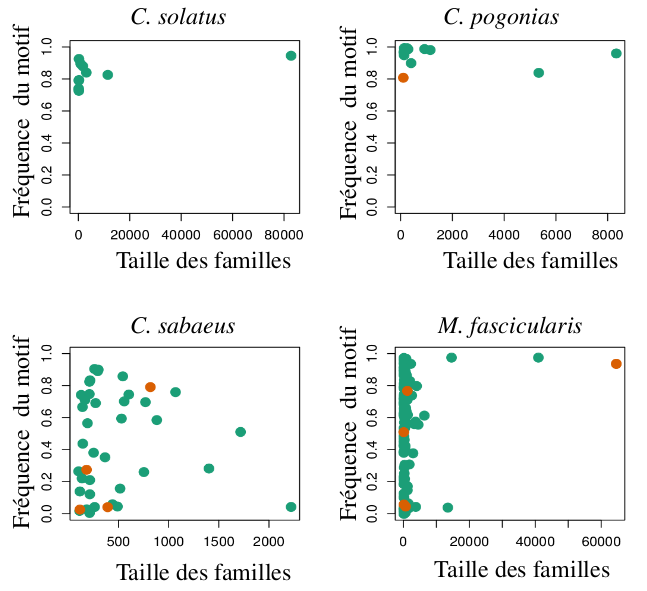
\includegraphics[scale=0.4]{img/graphique_motifs.png}
	\caption{\textbf{Présence des motifs CENP-B, pJ$\alpha$ ou pK$\beta$ par famille:}
	Le pourcentage de séquences par famille ayant le motif pJ$\alpha$ est en vert, pK$\beta$ en orange et CENP-B en bleu. Chaque famille est représentée en fonction de sa taille.
	\label{fig:motif}} 
\end{figure}
			La protéine CENP-B est présente chez toutes les espèces, mais les Cercopithèques ne possèdent pas son site de liaison. La protéine pJ$\alpha$ est une protéine peu connue mais dont le site de liaison est déterminé. Le motif pK$\beta$ est un site commun aux familles n'ayant ni CENP-B ni pJ$\alpha$. Ces trois motifs sont recherchés pour chaque famille de chaque espèce sur la base des consensus (partie matériel et méthodes) avec 2 mismatchs autorisés dans le but de caractériser ces familles. En effet, CENP-B est absent chez \textit{C. solatus} et \textit{C. pogonias}. Le \textit{C. sabaeus} et le \textit{M. fascicularis} n'ont pas ce motif non plus. Par contre plus de 90\% des familles chez les quatre espèces ont le motif pJ$\alpha$ mais à des niveaux différents.\\
		La totalité des familles chez \textit{C. solatus} ont le motif, dont 8 à plus de 75\%. Chez le \textit{C. pogonias}, 12 familles sur 13 ont le motif à plus de 75\%. Par ailleurs, la plus grande famille, C1, ayant plus de 80 000 séquences chez ces deux espèces, se démarque avec un pourcentage à 95\%. Le \textit{C. sabaeus} présente 39 familles avec ce motif, dont 7 l'ayant à plus de 75\%. Le \textit{M. fascicularis} a des pourcentages pour le motif pJ$\alpha$ qui varie entre 1\% et 97\%. Cette espèce a 28 familles avec le motif à plus de 75\% dont une famille de  40 000 séquences et une autre de 14 000 séquences.\\
			Le motif pK$\beta$ est présent lorsque pJ$\alpha$ est absent de la famille. Il est absent chez \textit{C. solatus}. Seule la famille C3 a ce motif à 80\% chez \textit{C. pogonias}. Le \textit{C. sabaeus} a quatre familles avec le motif, dont deux à 79\% et l'autre à 29\%. Le \textit{M. fascicularis} a cinq familles avec ce motif. La famille ayant le motif à 93\% est une grande famille de 64 000 séquences. Les deux autres familles ont le motif à 0.76\% et 0.50\%.\\
			Les quatre espèces ont des points en commun concernant l'absence du motif CENP-B et quelques familles ayant pK$\beta$. Cependant pour le motif pJ$\alpha$, les \textit{C. solatus} et \textit{C. pogonias}
 ont des pourcentages relativement proches mais qui diffèrent du \textit{M. fascicularis} et du \textit{C. sabaeus}, dont les valeurs sont intermédiaires. Chaque famille a un motif pour toutes les espèces excepté le \textit{M. fascicularis} qui a 6 familles sans motifs.\\ 			
			\subsubsection{Similarité entre familles}
\begin{figure}	
	\center
	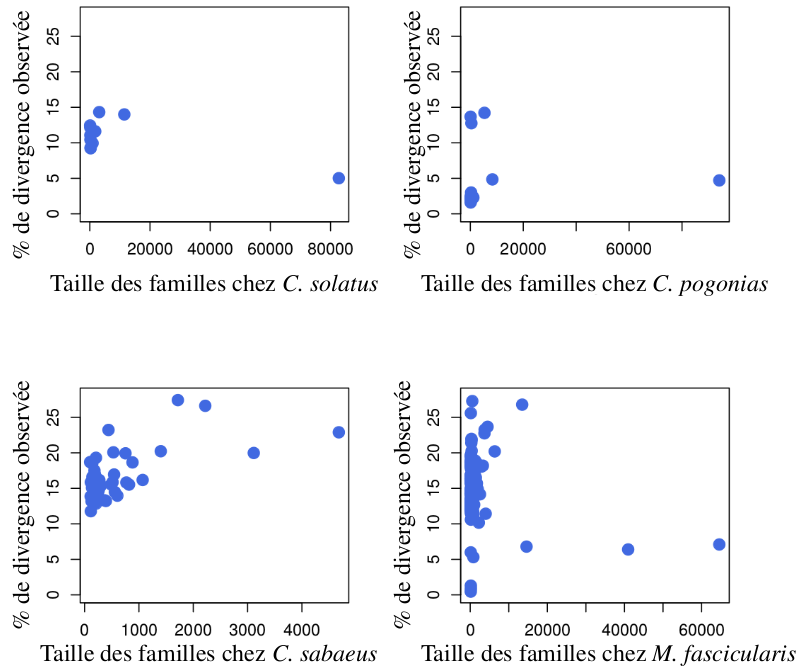
\includegraphics[scale=0.4]{img/graphique_similarity.png}
	\caption{\textbf{Pourcentage de divergence observée au sein d'une famille:}
	Un point correspond à une famille et son pourcentage de divergence observé.
	\label{fig:divergence}
		} 
\end{figure}
	Le pourcentage de divergence observée par famille est calculé sur 500 séquences tirées aléatoirement dans une famille pour estimer l'âge de celles-ci. Les \textit{C. solatus} et \textit{C. pogonias} ont des pourcentages relativement faibles ne dépassant pas 15\%, le \textit{M. fascicularis} a des valeurs intermédiaires variant de 0.1\% à 28\%, et \textit{C. sabaeus} a les valeurs les plus élevées allant de 11\% à 28\%.\\
	Les familles qui correspondraient aux familles C1 et C5 ont un pourcentage autour de 5\%. Les autres familles chez \textit{C. solatus} ont une moyenne de 10.85\%. Les familles de taille moyenne (quelques centaines de séquences) qui correspondraient à la famille C1 ont des pourcentages inférieurs à 3\% chez \textit{C. pogonias} et les trois familles restantes ont des valeurs de 13\% en moyenne. Les familles du \textit{C. sabaeus} ont en moyenne 16.8\% de divergence observée, la taille n'ayant aucun rapport au pourcentage. Le \textit{M. fascicularis} a trois familles avec un pourcentage inférieur à 1\% et cinq familles à 6\% en moyenne. Les 106 familles restantes ont un pourcentage supérieur à 10\%.\\
	Le pourcentage de similarité est semblable chez les \textit{C. solatus} et \textit{C. pogonias}. Le \textit{M. fascicularis} a  quelques familles qui ont le même comportement mais il a également beaucoup de familles aux pourcentages très élevés, tandis que la majorité des familles chez le \textit{C. sabaeus} a une grande partie de ses familles avec de grands pourcentages.
	

%########################################################################################################
	
	\subsection{Comparaison inter-espèce}
	Pour étudier les mécanismes d'évolution des $\alpha$-satellites, une classification inter-espèce ou "super-classification" (SC) permet de comprendre les différences entre espèces. Pour chaque espèce, 100 séquences par grande famille (> 100 séquences) sont tirées aléatoirement. Un jeu de données de 18 100 séquences est soumis à la classification automatique. A l'issue de cette super-classification, 158 familles sont obtenues au total, dont 90 grandes familles. Les petites familles de moins de 20 séquences, soit 1.76\% de ce jeu de données, ne sont pas prises en compte dans l'analyse.\\
	\subsubsection{Répartition des super-familles}
	Parmi les super-familles (SF), 38 ont une taille comprise entre 100 et 20 compris, et trois familles ont une taille strictement supérieure à 800 séquences. Seule une SF \textit{a priori} est commune aux quatre espèces. Elle rassemble 6 familles parmi les 10 familles classées C2 de \textit{C. solatus} et les deux familles également classées C2 de \textit{C. pogonias}, ainsi que deux familles du \textit{M. fascicularis} et une famille du \textit{C. sabaeus}. Une partie de la famille annotée C2 serait donc commune aux quatre espèces.\\
	Une SF est partagée entre le \textit{C. pogonias}, le \textit{C. sabaeus} et le \textit{M. fascicularis}. Cette SF regroupe des familles ayant le motif pK$\beta$ et qui correspondrait à la famille C3 commune au \textit{C. pogonias} et au \textit{C. solatus}. Cela signifierait que la famille C3 serait commune à ces quatre espèces également.\\
	Certaines SF sont spécifiques aux espèces. Au sein des 8 SF spécifiques du \textit{C. pogonias}, seule l'une d'entre elles regroupe deux familles, le reste étant composé d'une famille. Elles correspondraient aux familles C5, une petite partie de C6 et essentiellement à C1. Les trois SF spécifiques de \textit{C. solatus} seraient équivalentes aux familles C2. Le \textit{C. sabaeus} en a 3 et le \textit{M. fascicularis} 27.\\
	Le \textit{C. sabaeus} et le \textit{M. fascicularis} partagent 38 SF, soit 42\% des grandes SF (> 20 séquences), dont la plus grande faisant une taille de 1194 séquences. Une seule SF est uniquement commune à \textit{C. solatus} et \textit{C. pogonias} et elle regroupe les deux plus grandes familles qui seraient du C1.
	\subsubsection{Une mosaïque de familles C2}
			\begin{figure}
			\center	
			\begin{tabular}{cccc}
		\textbf{A.} & 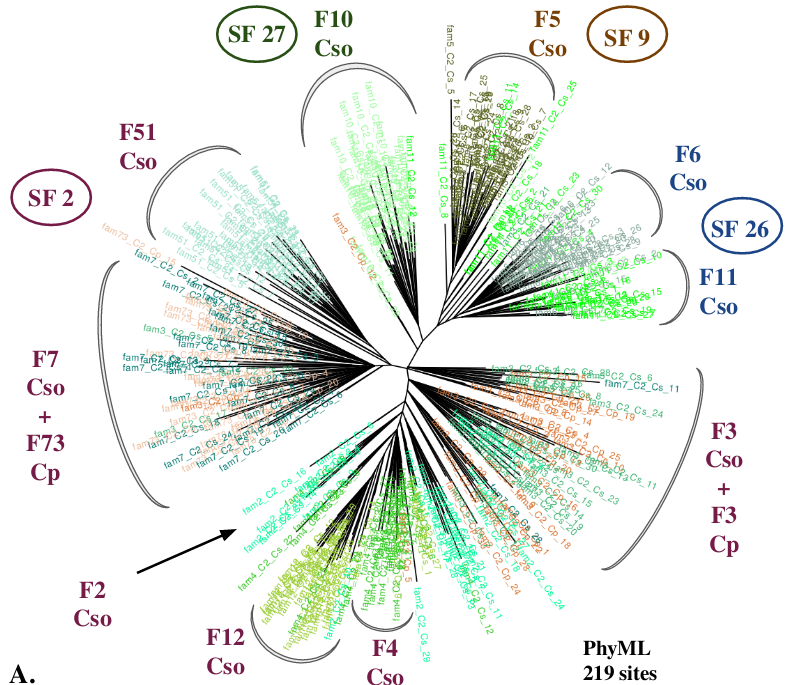
\includegraphics[scale=0.30]{img/tree_C2_pogonias_solatus.png} & \textbf{B.} & 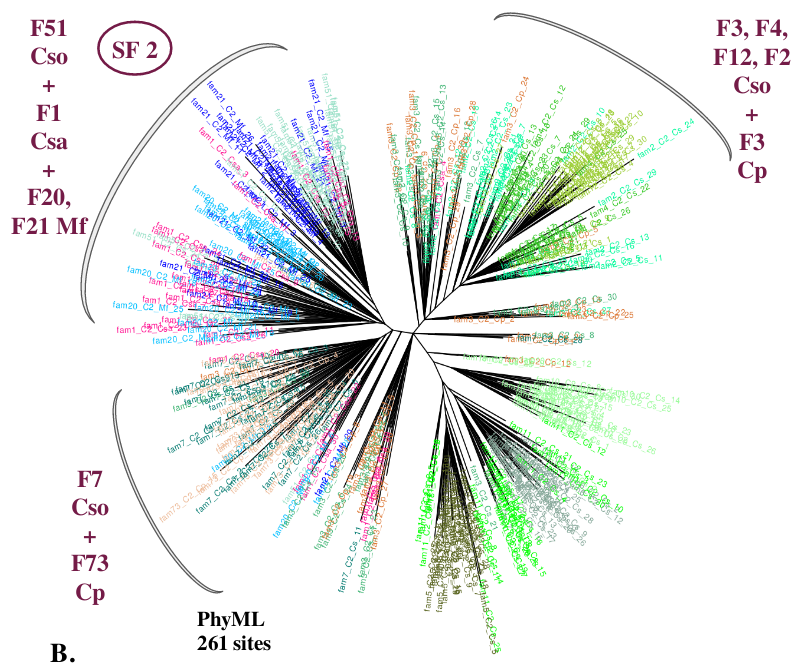
\includegraphics[scale=0.30]{img/tree_C2_all_species.png} \\
	\end{tabular}
	\caption{\textbf{Phylogénie des différentes familles qui correspondraient à la famille C2:}
	\textbf{A.}\textit{C. solatus} (tons verts) et \textit{C. pogonias} (tons orange) \textbf{B.} A ces deux espèces sont rajoutés des familles du \textit{M. fascicularis} (tons bleus) et \textit{C. sabeus} (rose).	 
	\label{tree_C2}
		} 
\end{figure}
		La famille C2 fait l'objet d'une séparation en plusieurs familles intéressante. Pour vérifier les résultats de cette SC, 30 séquences de chacune des familles C2 de \textit{C. solatus} et \textit{C. pogonias} sont tirées aléatoirement et un arbre est construit pour voir si cette division est retrouvée , puis un autre arbre avec les familles des deux autres espèces supposés de la famille C2 est rajouté au jeu de données précédent construit.\\
		Une partie de ces familles est spécifique au \textit{C. solatus}, tandis que les familles restantes sont communes aux quatre espèces selon la classification. Dans la phylogénie, les SF 27, 9 et 26 sont bien retrouvées. Cependant la SF 2 regroupe trop de familles, sans faire de distinction (Figure \ref{tree_C2} A). Les familles présumées C2 des deux autres espèces se mélangent plus spécifiquement avec la famille 51 de \textit{C. solatus}.							
	\subsubsection{Origine du motif pK$\beta$}
		\begin{figure}	
			\centering
				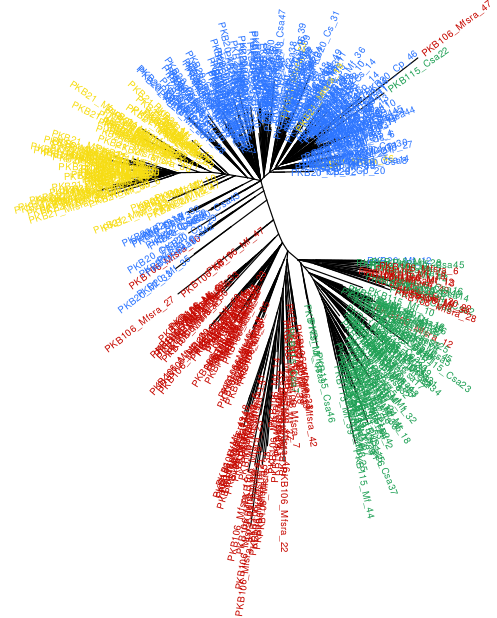
\includegraphics[scale=0.4, angle =90]{img/pkb_tree.png}				
				\caption{\textbf{Abre des super-familles pK$\beta$:} La super-famille 106 est en rouge, 115 en vert, 20 en bleu et 21 en jaunes.
	\label{fig:pkb_tree}} 
\end{figure}






	Pour poursuivre l'étude sur les familles communes entre espèces, le regroupement des familles $\alpha$-satellites ayant  le motif pK$\beta$ ou "familles pK$\beta$" attire l'attention. D'abord sont analysées les familles qui ont le motif à plus de 75\%. Elles représentent au mieux les familles pK$\beta$. Les familles qui expriment moins le motif sont analysées par la suite, pour voir si malgré la faible présence du motif, elles se rassemblent en une ou plusieurs super-familles.
	Le premier groupe de familles pK$\beta$ est constitué de la famille C3 de \textit{C. pogonias}, la famille 3 de \textit{C. sabeus}, et les familles 1 et 17 de \textit{M. fascicularis} qui expriment le motif à respectivement 80\%, 79\%, 94\% et 80\%. Ces familles s'assemblent en deux super-familles. La super-famille 21 est spécifique au macaque, regroupant la famille 1. La super-famille 20 regroupe les familles C3 de \textit{C. pogonias}, la famille 3 de \textit{C. sabeus} et la famille 17 de \textit{M. fascicularis}. Toutes ces espèces ont donc une "famille C3" en commun, peut-être sous forme de dimère C2-C3. Le deuxième groupe de famille pK$\beta$ est formé de la famille 27 de  \textit{C.sabeus} et les familles  47 et 294 du \textit{M. fascicularis} qui ont le motif à 27\%, 16\% et 41\% respectivement. La super-famille 106, regroupant la famille 294, est spécifique de \textit{M. fascicularis}. Les deux familles restantes, qui ont un faible pourcentage du motif, se regroupent pour former la super-famille 115. De plus, ces super-familles sont uniquement consitutées de familles pK$\beta$ et ne se mélangent pas aux autres familles.
	Un arbre composé de toutes les super-familles pK$\beta$ est construit pour voir comment elles s'assemblent. Le jeu de données est construit à partir de 50 séquences par famille pK$\beta$ par espèce tirées alétoirement (Figure \ref{fig:pkb_tree}) et contiennent la famille C3 de \textit{C. solatus}, dont la famille était trop petite pour être prise en compte. Comme les autres "familles C3", elle se range dans la super-famille 20. 

\section{Discussion}

	Les tailles moyennes des consensus sont de 173 nucléotides pour \textit{C. pogonias}, 173 pour \textit{C. solatus}, 173 pour le \textit{C. sabaeus} et X pour le \textit{M. fascicularis}\\
	
	Les plus grandes familles C2 de solatus sont regroupées\\


\section{Conclusion}

\newpage
\strut  ~  \mbox{}  \null
\newpage

\bibliographystyle{unsrt} \bibliography{biblio} 

%
%	\makeindex % index général
%   \newindex{env}{enx}{end}{Environnements}
%   \newindex{ext}{exx}{exd}{Extensions}
%   \newindex{cmm}{cmx}{cmd}{Commandes}
%	\newcommand{\commande}[1]
%   {\texttt{\textbackslash #1}}
%	\newcommand{\indexcmm}[1]
%   {\index[cmm]{#1@\commande{#1}}} % index d'une commande
% 
%
%
%
%Une citation\index{citation} hors paragraphe
%se met dans un environnement
%\emph{quote}\index[env]{quote}
%ou \emph{quotation}\index[env]{quotation}
% 
%L'extension \emph{array}\index[ext]{array}
%fournit les commandes
%\commande{raggedleft}\indexcmm{raggedleft}
%et \commande{raggedright}\indexcmm{raggedright}.
% 
%\printindex % index général
%\printindex[env]
%\printindex[ext]
%\printindex[cmm]

%%%%%%%%%%%%%%%%%%%%%%%%%%%%%%%%%%%%%%%%%%%%%%%%%%%%%%%%%%%%%%%%%%
%%%%%%%%%%%%%%%%%%%%Résumé & Abstract%%%%%%%%%%%%%%%%%%%%%%%%%%%%%
%%%%%%%%%%%%%%%%%%%%%%%%%%%%%%%%%%%%%%%%%%%%%%%%%%%%%%%%%%%%%%%%%%
\newpage 
\thispagestyle{empty}
\section*{Résumé}~\\[0.2cm]
Votre résumé commence ici...
   ...
\section*{Abstract}~\\[0.2cm]
 Abstract begins here...
   ...
\end{document}
%
%%HELP: http://lataix-sebastien.developpez.com/tutoriels/latex/memoire-de-fin-d-etude/#LII-C
